\chapter{Resultados e Validação}
\label{chap:resultados}

\begin{introduction}
Este capítulo apresenta os resultados obtidos, bem como a validação do sistema final de modo a garantir que cumpre com os requisitos pré-estabelecidos.
\end{introduction}

\section{Estado Final da Solução}

Após um período de desenvolvimento de vários meses, considero ter desenvolvido uma solução que cumpre com todos os objetivos e requisitos que defini no início deste projeto.

\subsection{Servidor}

O servidor consiste num ambiente de contentores (Docker Compose) que comunicam entre si, mantendo o isolamento necessário para que este sistema possa ser executado em cloud (caso desejado), ao mesmo tempo que permite a execução mais unificada do servidor em ambientes mais locais.

O principal ponto de acesso para ingestão de dados é um \textit{broker} Mosquitto (sendo que cada tópico com o prefixo \texttt{sensors/} é considerado um tipo de sensor diferente) que permite a ingestão unificada de dados de vários utilizadores. Estes registos são depois transferidos para o Kafka (que possui melhor resiliência de dados) de forma automática e agnóstica via Kafka Connect antes de serem inseridos de forma assíncrona na base de dados (novamente usando Kafka Connect), onde cada tópico \ac{MQTT} é inserido numa tabela (\textit{measurement}) distinta no InfluxDB. Esta abordagem agnóstica e aberta permite não só acrescentar sensores sem ter de modificar o servidor, mas também a possibilidade de integrar com sistemas pré-existentes (necessitando apenas de usar o prefixo "sensors/" no tópico e incluir \texttt{uuid} e \texttt{timestamp} na mensagem).

O acesso da base de dados por parte dos clientes é gerido por uma API REST simples (escrita em FastAPI). O endpoint principal desta API é \texttt{/data/{sensor}}, que constroi uma \textit{query} para um sensor específico a partir dos seguintes parâmetros:
\begin{itemize}
    \item \textbf{start e end}: janela temporal, em ms, para a qual queremos obter os dados.
    \item \textbf{uuid}: o \ac{UUID} do utilizador a que pertecem os dados.
    \item \textbf{agg}: o tipo de agregação (opcional) (MEAN, COUNT, SUM, MIN, MAX). Por defeito (ou se utilizar NONE), os valores não são agregados.
    \item \textbf{field}: o campo (ou campos, separados por vírgula) a retornar. O valor por defeito é \texttt{value}.
    \item \textbf{interval}: o intervalo de tempo (opcional) para agregação (deverá incluir o valor e a unidade de tempo, por exemplo \texttt{1s}). Se omitido os valores não são agregados por tempo.
\end{itemize}
O uso desta API e de parâmetros evita que agentes externos tenham acesso à base de dados, reduzindo por isso o risco de vulnerabilidades.

\subsection{Cliente}

A aplicação para \textit{desktop} foi criada para ser simultaneamente uma demonstração das capacidades do sistema e de como interagir com este para quem deseje criar o seu próprio \textit{frontend}, mas também uma base funcional que permite integrar de forma célere novos tipos de sensores, conforme as necessidades de cada investigação.

De modo a facilitar a extensão, a app utiliza um sistema de \textit{plugins} com uma interface pré-estabelicida, divididos em dois tipos principais: \textit{plugins} de sensores e \textit{plugins} de visualização.
\begin{itemize}
    \item \textbf{\textit{Plugins} de sensores:} são responsáveis pela interação direta (ou indireta no caso de sensores externos) com os sensores, recolhendo informações. Os sensores podem ser controlados de forma unificada (selecionar os sensores pretendidos e começar/parar a recolha de dados) a partir de um painel de controlo (ver Figura~\ref{fig:painel_controlo}). Para demonstrar a recolha de dados, foram criados 3 \textit{plugins} para sensores distintos (2 internos e 1 externo): um para controlo da app para WearOS (\ac{HRV}), um para obter direção do olhar e grau de abertura dos olhos via \textit{webcam} e outro para registar a cadência e o tipo de teclas premidas num teclado.
    \item \textbf{\textit{Plugins} de visualização:} atuam na camada da interface, sendo responsáveis por consumir os dados obtidos via API REST de um ou mais sensores e transformá-los em representações gráficas (ver Figura~\ref{fig:hrv}). No caso de gráficos de linha, será necessário apenas implementar métodos para a recolha e tratamento dos dados, sendo que a visualização destes já está estabelecida na classe que herdam. Foram criados 3 \textit{plugins} de visualização: dois focados na visualização direta de dados de um sensor (\ac{HRV} e caracteres por minuto) e outro que utiliza os dados dos 3 sensores para estimar o nível de atenção.
\end{itemize}

\begin{figure}[H]
     \centering
     \begin{subfigure}[b]{0.48\textwidth}
         \centering
         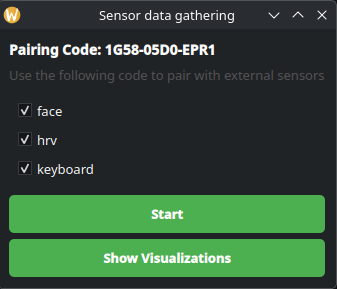
\includegraphics[width=\linewidth]{figs/desktop/desktop_painel.png}
         \caption{Painel de controlo dos sensores}
         \label{fig:painel_controlo}
     \end{subfigure}
     \hfill % Cria um espaço elástico entre as duas imagens
     \begin{subfigure}[b]{0.48\textwidth}
         \centering
         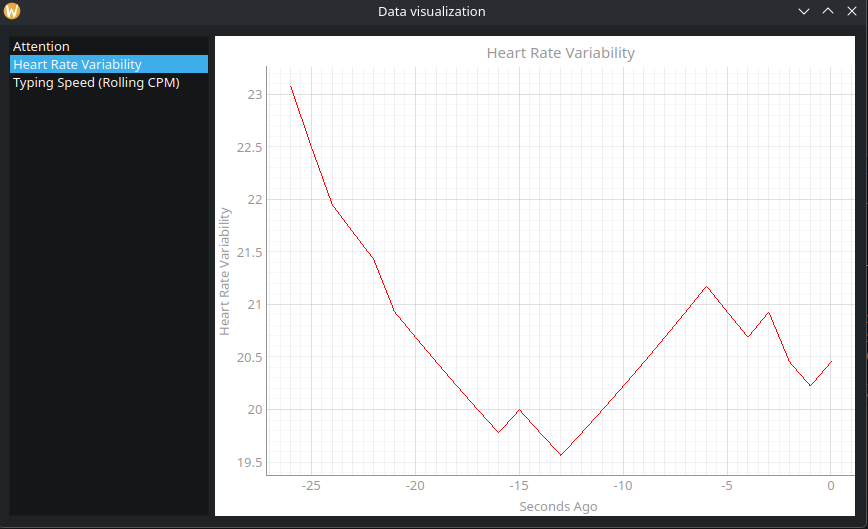
\includegraphics[width=\linewidth]{figs/desktop/desktop_grafico_hrv.png}
         \caption{Painel de visualização (hrv)}
         \label{fig:hrv}
     \end{subfigure}
     \caption{Interface da aplicação para \textit{desktop}}
\end{figure}

\subsection{App de WearOS}

A aplicação para WearOS foi criada para exemplificar a recolha de dados usando sensores externos (neste caso, um \textit{smartwatch}), a aplicação utiliza o \textit{broker} \ac{MQTT} local para comunicação e controlo (via um \textit{plugin} da app para \textit{desktop}), sendo que o funcionamento pode-se dividir em 5 etapas.
\begin{enumerate}
    \item \textbf{Emparelhamento} (Figura~\ref{fig:wearos_pairing}): Durante a primeira inicialização (ou quando mudar o endereço IP), o utilizador insere um código de 12 dígitos que contém informações sobre o endereço IP e porta aos quais vai ter de subscrever para receber comandos. Este código é gerado automaticamente pela app para \textit{desktop} através de Crockford Base64 (um método de codificação que elimina caracteres similares para reduzir erros de digitação) e está presente no painel de controlo da app.
    \item \textbf{Estabelecimento de conexão} (Figura~\ref{fig:wearos_connecting}): Ecrã mostrado até ao estabelecimento da conexão com o \textit{broker} MQTT.
    \item \textbf{Escuta de comandos} (Figura~\ref{fig:wearos_waiting}): Ecrã mostrado após a conexão, permanecendo ativo até à receção do sinal de início de sessão (ou após a interrupção da mesma).
    \item \textbf{Inicialização de sensores} (Figura~\ref{fig:wearos_preparing}): Ecrã mostrado após o começo da sessão, caso os sensores ainda não estejam prontos. Como a preparação dos sensores começa ao iniciar a aplicação, esta fase é frequentemente omitida.
    \item \textbf{Envio de dados} (Figura~\ref{fig:wearos_sending}): Ecrã mostrado durante o envio de dados, indicando também o valor a ser enviado (bem como o número de batimentos por minuto para referência). 
\end{enumerate}

\begin{figure}[H]
     \centering
     \begin{subfigure}[t]{0.19\textwidth}
         \centering
         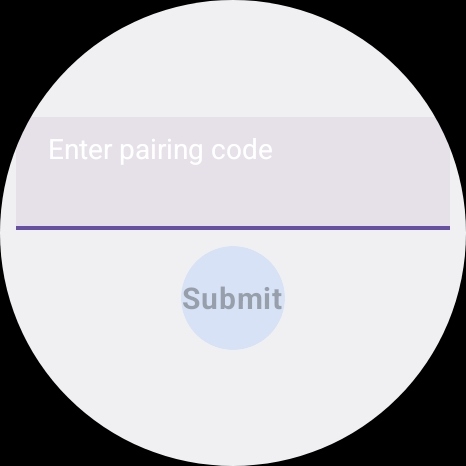
\includegraphics[width=\linewidth]{figs/wearos/wearos_pairing}
         \caption{Emparelhamento}
         \label{fig:wearos_pairing}
     \end{subfigure}
     \hfill
     \begin{subfigure}[t]{0.19\textwidth}
         \centering
         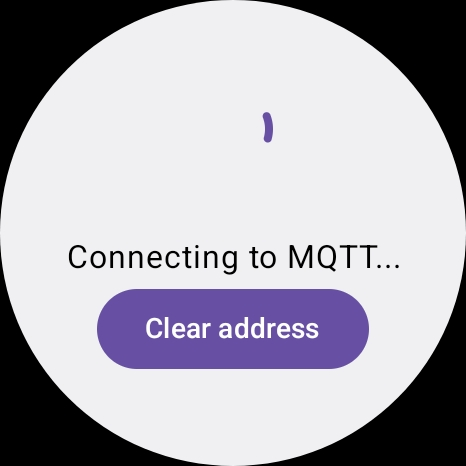
\includegraphics[width=\linewidth]{figs/wearos/wearos_connecting}
         \caption{Estabelecimento de Conexão}
         \label{fig:wearos_connecting}
     \end{subfigure}
     \hfill
     \begin{subfigure}[t]{0.19\textwidth}
         \centering
         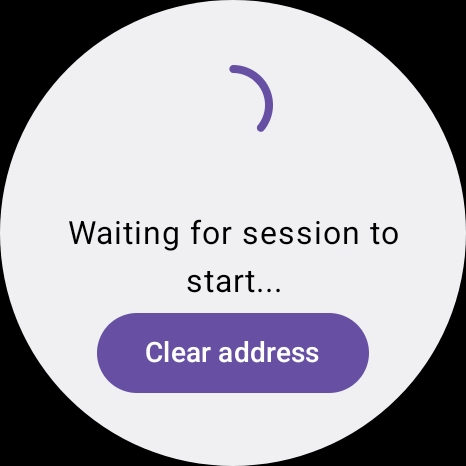
\includegraphics[width=\linewidth]{figs/wearos/wearos_waiting}
         \caption{Escuta de comandos}
         \label{fig:wearos_waiting}
     \end{subfigure}
     \hfill
     \begin{subfigure}[t]{0.19\textwidth}
         \centering
         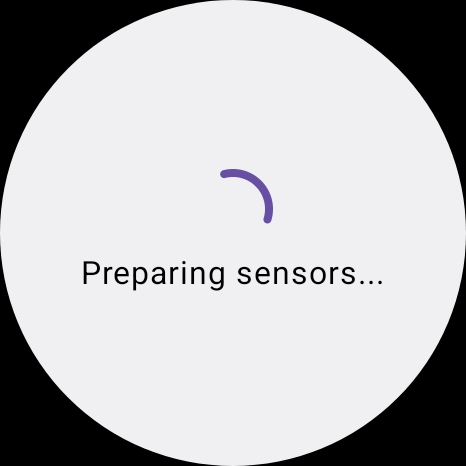
\includegraphics[width=\linewidth]{figs/wearos/wearos_preparing}
         \caption{Inicialização de sensores}
         \label{fig:wearos_preparing}
     \end{subfigure}
     \hfill
     \begin{subfigure}[t]{0.19\textwidth}
         \centering
         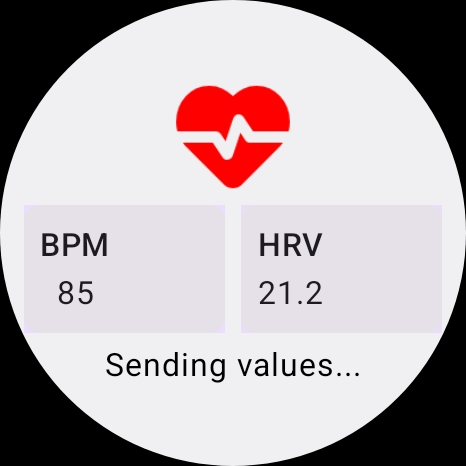
\includegraphics[width=\linewidth]{figs/wearos/wearos_sending}
         \caption{Envio de dados}
         \label{fig:wearos_sending}
     \end{subfigure}     
     \caption{Interface da aplicação para WearOS}
\end{figure}

\subsection{Fluxo de Dados}

De modo a ilustrar como estes componentes comunicam entre si, a Figura~\ref{fig:end2end} mapeia o fluxo de dados \textit{end-to-end}, utilizando como exemplo os dados faciais obtidos via \textit{webcam}:

\begin{enumerate}
    \item \textbf{Captura e ingestão:} O \textit{plugin} da \textit{webcam} presente na aplicação \textit{desktop} captura uma \textit{frame} e extrai as \textit{features} faciais (utilizando a biblioteca MediaPipe). Essas \textit{features} são convertidas em métricas (de modo a reduzir o volume de dados a enviar) e enviadas para o \textit{broker} Mosquitto local.
    \item \textbf{Redirecionamento:} Os dados presentes no broker local (em tópicos com o prefixo \texttt{sensors/}) são redirecionados para um \textit{broker} remoto automaticamente.
    \item \textbf{Transporte:} Após a chegada de novos dados ao \textit{broker}, o conector \textit{source} do Kafka Connect recolhe estes dados e insere-os no Kafka (que possui melhor resiliência que o Mosquitto, permitindo ingestão assíncrona).
    \item \textbf{Armazenamento:} Após a inserção no Kafka, um segundo conector \textit{sink} de Kafka Connect consome as mensagens e armazena-as na base de dados.
    \item \textbf{Acesso e visualização:} Após o armazenamento dos dados, estes são acedidos via API REST pela app \textit{desktop} a cada segundo para gerar uma visualização dos dados.
\end{enumerate}

\begin{figure}
    \centering
    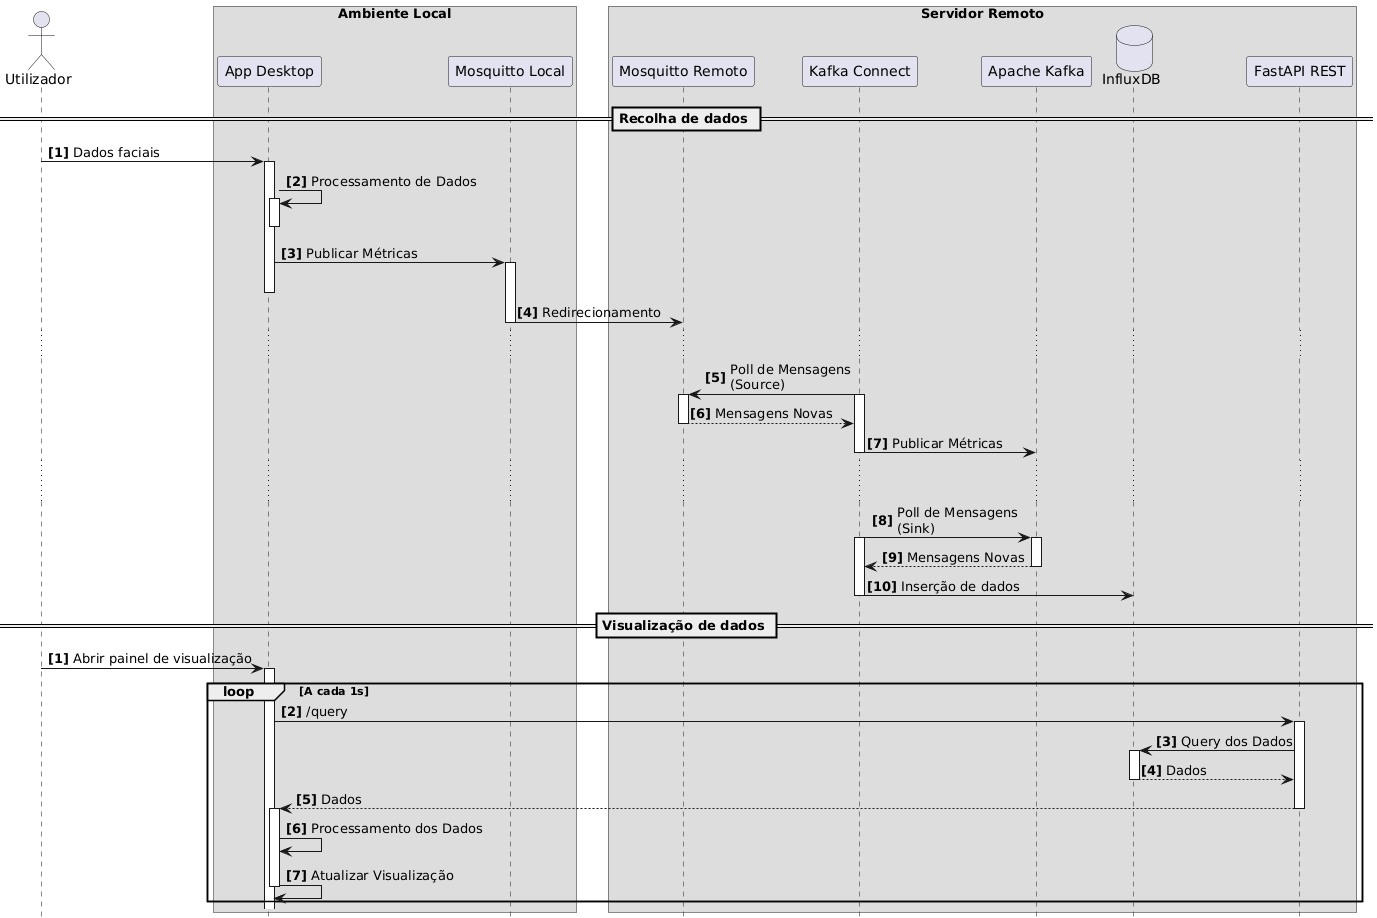
\includegraphics[width=\linewidth]{figs/end2end.png}
    \caption{Fluxo de dados \textit{end-to-end}}
    \label{fig:end2end}
\end{figure}